\documentclass{uflamon}          % classe base para a monografia

%==============================================================================
% Utilizacao de pacotes
\usepackage[T1]{fontenc}         % usa fontes postscript com acentos
\usepackage[brazil]{babel}       % hifenização e títulos em português do Brasil
\usepackage[utf8]{inputenc}     % permite edição direta com acentos
\usepackage{amsmath}             % pacote da AMS para Matemática Avançada
\usepackage{amssymb}             % símbolos extras da AMS
\usepackage{latexsym}            % símbolos extras do LaTeX
\usepackage{graphicx}            % para inserção de gráficos
\usepackage{listings}            % para inserção de código
\usepackage{fancyvrb}            % para inserção de saídas de comandos
%\usepackage{enumerate}           % para personalizar lista enumeradas 
											%(incluso na classe)
\usepackage{longtable}           % para tambelas muito grandes NOVO!!!!

\usepackage{colortbl} % cores em tabelas
\newcolumntype{Z}{|>{\columncolor[gray]{0.9}}l|} %cor cinza em células
%\usepackage{array} % já incluso na classe
\newcolumntype{L}[1]{>{\raggedright\let\newline\\\arraybackslash\hspace{0pt}}m{#1}}
\newcolumntype{C}[1]{>{\centering\let\newline\\\arraybackslash\hspace{0pt}}m{#1}}
\newcolumntype{R}[1]{>{\raggedleft\let\newline\\\arraybackslash\hspace{0pt}}m{#1}}
\usepackage{multirow} % para juntar duas linhas em uma só

\usepackage{multicol} % para uso de várias colunas

% cores para os links cruzados
\usepackage{color}
\definecolor{rltred}{rgb}{0.2,0,0}
\definecolor{rltgreen}{rgb}{0,0.2,0}
\definecolor{rltblue}{rgb}{0,0,0.2}

\usepackage[colorlinks=true,
            urlcolor=rltblue,       % \href{...}{...} external (URL)
            filecolor=rltgreen,     % \href{...} local file
            linkcolor=rltred,       % \ref{...} and \pageref{...}
            citecolor=rltgreen,
            pdftitle={Exemplo de Uso da Classe Uflamon},
          pdfauthor={Gustavo Costa Neves},
          pdfsubject={Este texto tem por objetivo servir de exemplo da classe Uflamon.},
          pdfkeywords={Comunicação Científica. 2. Pesquisa . 3. Pesquisa Científica. 
 					 4. Redação. 5. Monografia.}%
]{hyperref} % para referência cruzadas
%\usepackage{hyperref}            % para referência cruzadas
\usepackage{subfigure}           % figuras dentro de figuras
\usepackage{caption}            % remodelando o formato dos títulos de 
                                 % tabelas e figuras

% configuração padrão do listings   
\lstset{
   language=Java,
   extendedchars=true,
   tabsize=3,
   basicstyle=\footnotesize\ttfamily,
   stringstyle=\em,
   showstringspaces=false 
}

% para referências de acordo com a ABNT
% precisa instalar o abntex2 antes!!!
% http://abntex.codigolivre.org.br/
% comente se pretende usar outro padrão

%abnt-emphasize=bf coloca o título das bibliografias em negrito
%abnt-thesis-year=both
\usepackage[alf,abnt-etal-cite=3,abnt-etal-list=3,abnt-url-package=url,abnt-emphasize=bf]{abntex2cite}

% evite usar o hyperref com abntex, pode dar caca em urls... no linha anterior, informo
% para incluir urls usando o pacote url e não o hyperref
%
% caso queira o hyperref com abntex, comente a linha anterior e descomente a seguinte
%\usepackage[alf,abnt-etal-cite=3,abnt-etal-list=0,abnt-etal-text=emph]{abntex2cite}
%
% caso vc ainda use a versão anterior da abntex, comente a linha incluindo o abntex2cite
% e descomente a próxima linha 
%\usepackage[alf,abnt-etal-cite=3,abnt-etal-list=0,abnt-etal-text=emph]{abntcite}


% redefinindo formatação de títulos de tabelas e figuras


%==============================================================================
% para os fãs do Word, descomente as linhas abaixo
%\sloppy %mais espaço entre as linhas
%\usepackage{identfirst} %identando-se a primeira linha de cada seção
%\noindentfirst % Tire o comentário para manter o padrão do LaTeX.

%==============================================================================
% definido comandos na monografia - não é necessário na sua monografia 
% apenas para exemplificar a definição de novos comandos
\newcommand{\defs}[1]{\textsl{#1}}


% Especificando hifenizações que por ventura LaTeX não saiba fazer
% Por padrão 99,9% dos termos em português devem ser hifenizados corretamente.
\hyphenation{hardware software Li-nux am-bien-te diag-nos-ti-car coor-de-na-ção 
FAE-PE Recovery TelEduc Williams UFLA}

%==============================================================================
% Dados da monografia, capa: autor, titulo, banca, etc... - SUBSTITUA DE ACORDO
%==============================================================================
\author{Gustavo Costa Neves}
\title{ESTÁGIO EM DESENVOLVIMENTO DE SISTEMAS WEB NO LEMAF/UFLA}
\engtitle{Use of Uflamon Class}
\engsubtitle{Sample for Users}
\date{2019}
\tipo{Relatório de estágio apresentado na
Universidade Federal de Lavras – UFLA
como requisito para obtenção do título de
graduação no curso de Ciência da computação, sob orientação da Professora
Marluce Rodrigues Pereira.
}
% use \orientador ou \orientadora quando for o caso
\orientadora{Prof. Marluce Rodrigues Pereira}
%\orientadora{}
% use \coorientador ou \coorientadora quando for o caso
%\coorientadora{Prof. DSc. Maria Orientadora } % comente se não tiver coorientador
%\coorientador{}
\local{Lavras -- MG}
\bancaum{Prof. MSc. Antônio Banca Um}{UFM}
\bancadois{Prof. DSc. João Banca Dois}{FCO} % comente se sua banca tiver só um professor
\bancatres{Profa. Esp. Eliza Banca Três}{BELMIS}
\bancaquatro{Prof. Esp. Carlos Banca Quatro}{IBGPLUS}
\defesa{30 de Fevereiro de 2019}
%==============================================================================


%##################################################

%\antesfichacat{\noindent Para citar este documento: \\UNIVERSIDADE FEDERAL DE LAVRAS. Biblioteca Universitária. \textbf{Manual de normalização e estrutura de trabalhos acadêmicos: TCC, monografias, dissertações e teses}. 2. ed. rev., atual. e ampl. Lavras, 2015. Disponível em: \url{http://www.biblioteca.ufla.br/wordpress/wpcontent/uploads/bdtd/manual_normalizacao_UFLA.pdf}. Acesso em: data de acesso.}

%\depoisfichacat{\noindent A reprodução e a divulgação total ou parcial deste trabalho são autorizadas, por qualquer meio convencional ou eletrônico, para fins de estudo e pesquisa, desde que citada a fonte.\\
%\newline
%{\small Este documento possui páginas em branco para facilitar a impressão frente-e-verso.}}

%##################################################

%##################################################

% para os exemplos do manual
%\newenvironment{exemplomanual}{
%\vspace{0.5cm}
%\noindent\begin{minipage}{\textwidth}
%\noindent\rule{\textwidth}{0.5pt}
%\vspace{-1cm}
%\begin{flushleft}
%}{
%\end{flushleft}
%\vspace{-0.6cm}
%\noindent\rule{\textwidth}{0.5pt}
%\vspace{0.3cm}
%\end{minipage}
%}

%\newenvironment{exemplomanuallista}{
%\vspace{0.3cm}
%\noindent\begin{minipage}{\textwidth - 0.5cm}
%\noindent\rule{\textwidth}{0.5pt}
%\vspace{-1cm}
%\begin{flushleft}
%}{
%\end{flushleft}
%\vspace{-0.6cm}
%\noindent\rule{\textwidth}{0.5pt}
%\vspace{0.3cm}
%\end{minipage}
%}

% por conta de alguns exemplos
%\usepackage{setspace}

%##################################################

% se vc já defendeu e tem o arquivo escaneado da folha de rosto, 
% descomente e altere o nome do arquivo
%\folhaAprovacaoAssinada{folharosto}

% Aqui começa o documento propriamente dito
\begin{document}

\maketitle

\dedic{Dedico esse trabalho de conclusão de curso aos meus pais que sempre me apoiaram em toda essa tragetória}     % Dedicatórias\\

\thanks{Agradeço a todos que estiveram contribuindo comigo durante esse periodo de ufla.
\\
\\
Agradecimentos especiais para: 
\\

\quad Bruna Gomes.

\quad Danilo Guarizzo.

\quad Ivan Carvalho.

\quad Bruno Custódio.

\quad Highlander Silva.

\quad Matheus Flausino.

\quad Amanda Lima.

\quad Todos funcionarios do LEMAF que trabalhei junto.}         % Agradecimentos

% palavras-chave
\palchaves{Processos agéis, Desenvolvimento web, Frameworks.}
\resumo{Este relatório de estágio descreve as atividades desenvolvidas no Laboratório de Projetos e Estudos em Manejo Florestal – LEMAF. O estágio descrito neste relatório teve duração de 1 ano e teve como objetivo o desenvolvimento de sistemas e ferramentas para controle e manejo ambiental.
O relatório visa descrever os processos de desenvolvimento dentro da empresa, como metodologias ágeis, estágios de desenvolvimento (prototipação, design system, desenvolvimento, homologação) e organização no geral. Desta forma, o trabalho tem como objetivo relatar a experiência como desenvolvedor estagiário no LEMAF.}
% keywords devem vir antes do abstract
\keywords{Agile Processes, Web Development, Frameworks.} % keywords
\abstract{This internship report describes how activities are carried out at the Forest Management Project - LEMAF. The internship described in this report lasted one year and aimed to develop systems and tools for environmental control and management. 
The report aims to describe the development processes within the company, such as methodologies, development steps (prototyping, system design, development, approval) and overall organization. Thus, the work aims to report an experience as a trainee developer at LEMAF.}% ################################ ##################
% Dados do guia
%\begin{titlepage}
%\pagestyle{empty}
%\renewcommand{\baselinestretch}{1}
%\enlargethispage{1.5cm}
%\input{reitoria}
%\cleardoublepage
%\end{titlepage}

%##################################################

% descomente para habilitar a lista desejada
\listoffigures                             % Lista de Figuras
%\listofilustracoes
%\listofgraficos							   % Lista de Gráficos
%\listoftables                              % Lista de Tabelas
%\listofquadros							   % Lista de Quadros
%\listofexemplos
%\listofteoremas
\tableofcontents                           % Sumário

\clearpage

\pagestyle{ufla}

%==============================================================================
% incluindo os capitulos
\chapter{INTRODUÇÃO}
\label{cap:introducao}

Este trabalho visa apresentar as experiências vividas durante o período como estagiário do LEMAF (Laboratório de Projetos e Estudos
em Manejo Florestal), laboratório situado dentro da Universidade Federal de Lavras (UFLA) onde são desenvolvidas soluções tecnológicas relacionadas a manejo florestal.
O laboratório foi inaugurado em 2002 e, desde lá, desenvolve diversos projetos para órgãos governamentais e empresas privadas, contando em 2018 com mais de 100 funcionários.

Os projetos do LEMAF geralmente possuem contextos relacionados à preservação ambiental, como monitoramento de áreas desmatadas e uso indevido de recursos hídricos. Porém sua carteira de projetos inclui diversos temas, como portais para povos indígenas, monitoramento de número de animais atropelados em determinada região e até mesmo gerenciadores de conteúdos.   
O estágio proporcionado pelo mesmo tinha como responsabilidades o seguimento de metodologias ágeis, organização, trabalho em equipe e, principalmente, o desenvolvimento de projetos web.

Por conta de uma grande rotação de projetos e times, foi necessário o estudo de diversos frameworks e tecnologias, onde os principais relacionados com frontend foram Angular, Vuejs e ReactJs, enquanto com backend foram SpringBoot, DotNet Framework e PlayFramework.
Para que o desenvolvimento dos projetos fluíssem efetivamente, eram utilizadas diversas metodologias ágeis, como principais Scrum e Kanban.

Com toda essa carga de conhecimento e responsabilidades, ser estagiário no LEMAF se tornou uma experiencia incrível. Estava sempre evoluindo, conhecendo novas tecnologias do mercado e tendo oportunidade de obter conhecimento de pessoas extremamente experientes no ramo.

Os demais capítulos deste relatório estão organizados da seguinte forma.  No Capítulo 2 são abordadas as ferramentas e processos utilizados durante o estágio. No Capítulo 3 são apresentadas e discutidas as principais tecnologias utilizadas durante o estágio. No Capítulo 4 são apresentadas as atividades desenvolvidas durante o estágio. No Capítulo 5 são apresentadas conclusões.
\chapter{ELEMENTOS DO TEXTO}
\label{cap:elementos}

Graças ao grande numero de termos específicos da área de desenvolvimento, é necessária a explicação dos mesmos.

\section{Metodologias Ágeis}

\subsection{Scrum}

Metodologia ágil que visa ter escopo fechado(numero de tarefas predefinidas), calculadas através de métricas da equipe, como pontos de esforço.

Muitas vezes separadas em Sprints(tempo pre-definido pela equipe, geralmente de 10 dias utéis), as tarefas são incluídas em um quadro e devem ser finalizadas ate o fim do prazo.

\begin{quote}
  O framework Scrum consiste nos times do Scrum associadas a papéis, eventos, artefatos e
  regras. Cada componente dentro do framework serve a um propósito específico e é essencial
  para o uso e sucesso do Scrum.
\end{quote}

\subsection{Kanbam}
  Opção de metodologia ágil mais adaptativa, tendo escopo aberto torna-se possível inserir atividades durante o tempo.
  Geralmente se é determinado um máximo de esforço e ao final de alguma atividade, é inserida uma nova com prioridade.
\begin{figure}[!htb]
\centering
\caption{Quadro kanbam} %legenda
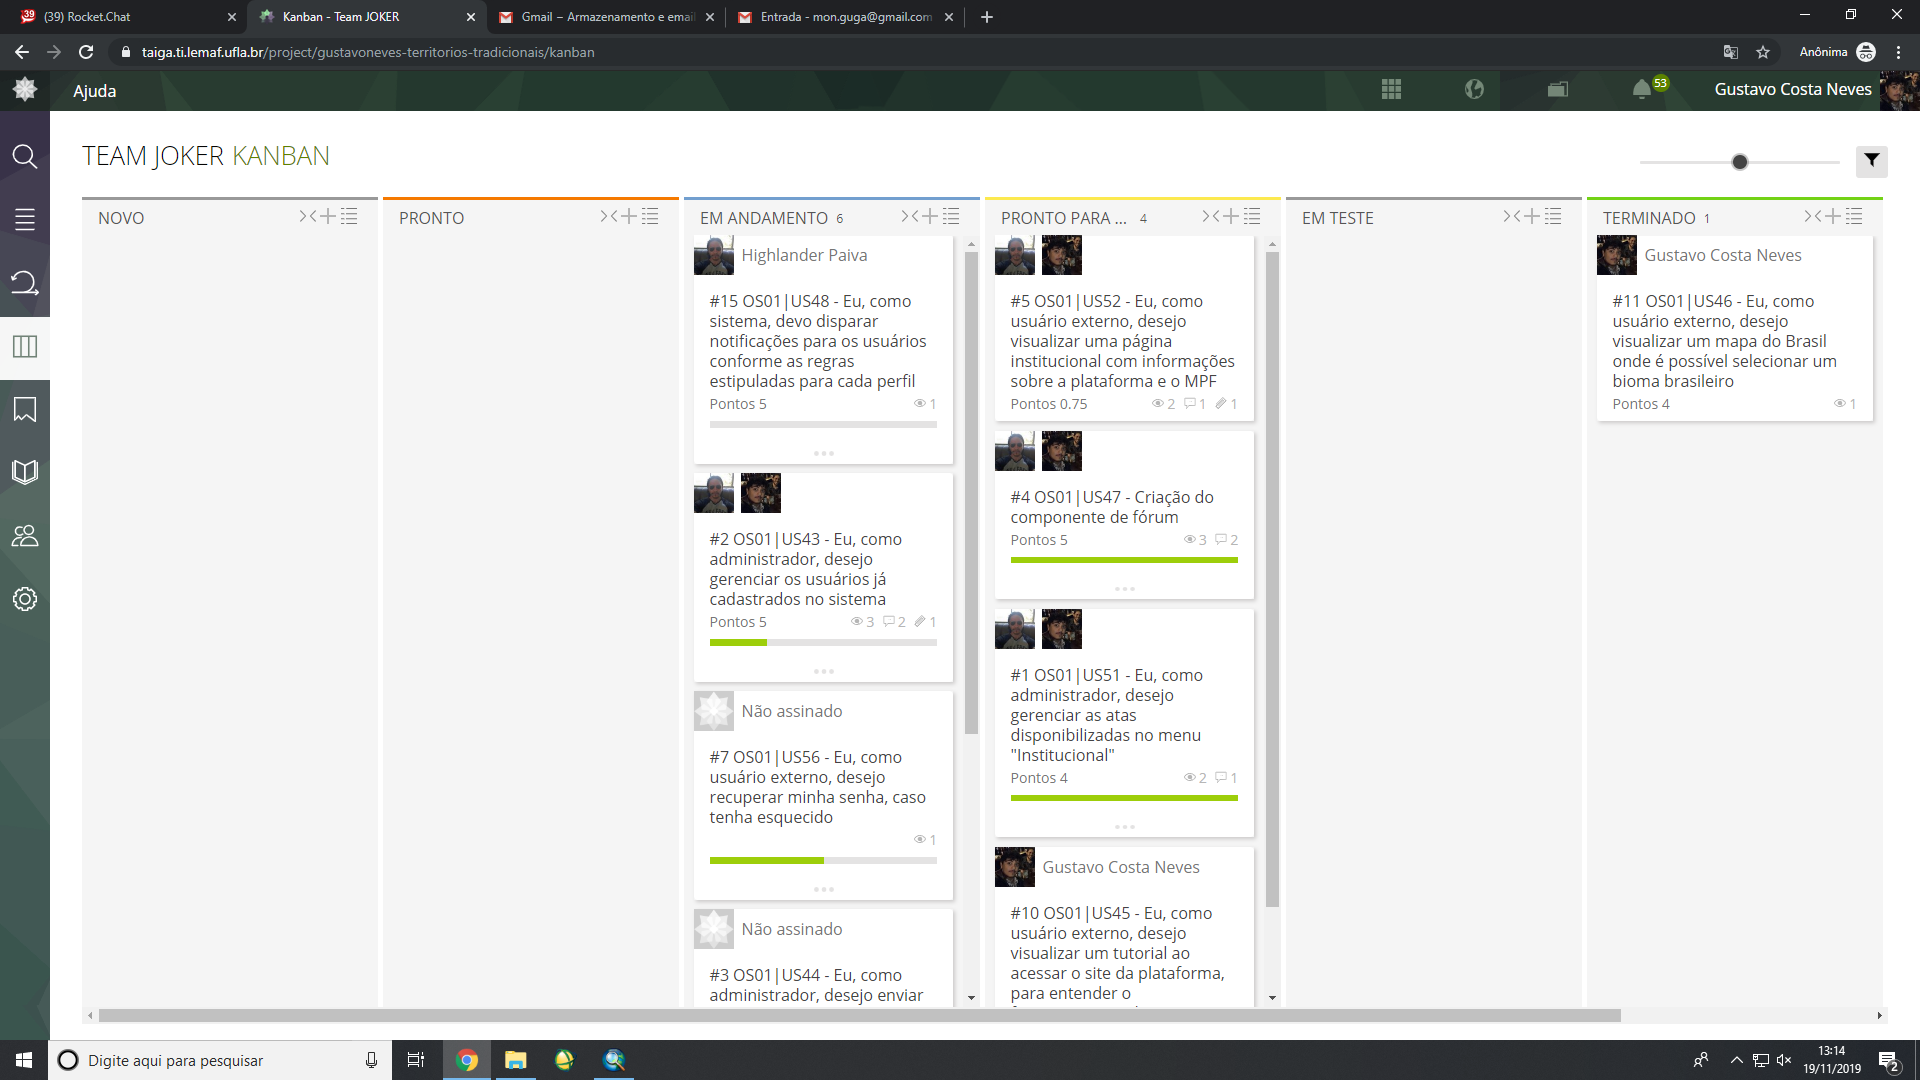
\includegraphics[scale=0.2]{quadroKanbam}\\  % o 0.9 indica 90% do tamanho original
% pdfLaTeX aceita figuras no formato PNG, JPG ou PDF
% figuras vetoriais podem ser exportadas para eps e depois convertidas para pdf usando epstopdf
{\small Fonte: https://taiga.ti.lemaf.ufla.br/} %Fonte da imagem
\label{fig:exemplo} %rotulo para refencia
\end{figure}

\section{Frameworks}

Para facilitar o desenvolvimento, diversas ferramentas já foram criadas e durante o desenvolvimento de novos projetos, foi necessária a utilização das mesmas.

\subsection{Frontend}

É a parte da aplicação que interage diretamente com o usuário.

\subsubsection{Angular}

Angular é um framework open-source de desenvolvimento front-end que possibilita o desenvolvimento de aplicações web.

Teve sua primeira versão foi lançada em 2016.

\subsubsection{VueJS}

Vue.js é um framework JavaScript de código-aberto, focado no desenvolvimento de interfaces de usuário e aplicativos de página única

Teve sua primeira versão lançada em 2014.

\subsubsection{ReactJS}

O React é uma biblioteca JavaScript de código aberto com foco em criar interfaces de usuário em páginas web. É mantido pelo Facebook, Instagram, outras empresas e uma comunidade de desenvolvedores individuais. 

Teve sua primeira versão lançada em 2013.

\subsection{Backend}

É a parte da aplicação que fica escondida do usuário, é onde é controlado todo o sistema(autenticação, regras de negocio, jobs e etc).

\subsubsection{PlayFramework}

O Play Framework é uma alternativa "limpa" de esticar as stacks do Java Enterprise. Ele se concentra na produtividade do desenvolvedor e tem como objetivo arquiteturas RESTful. O Play é um companheiro perfeito para o desenvolvimento ágil de software.

O objetivo da estrutura do Play é facilitar o desenvolvimento de aplicativos da web, mantendo o Java.

Teve sua primeira versão lançada em 2009.

\subsubsection{Spring Boot}

O Spring é um framework open source para a plataforma Java criado por Rod Johnson e descrito em seu livro "Expert One-on-One: JEE Design e Development". Trata-se de um framework não intrusivo, baseado nos padrões de projeto inversão de controle e injeção de dependência.

Teve sua primeira versão em 2002.

\subsubsection{DotNet Framework}

O .NET Framework é uma iniciativa da empresa Microsoft, que visa uma plataforma única para desenvolvimento e execução de sistemas e aplicações. Todo e qualquer código gerado para .NET pode ser executado em qualquer dispositivo que possua um framework de tal plataforma.

Teve sua primeira versão lançada em 2002.

\section{Cargos}

Para melhor organização dos projetos, os funcionários são separados em tribos e squads com alguns cargos específicos para cada integrante.

\subsection{Scrum Master}

Cargo que tem como função cuidar das obrigações impostas sobre a metodologia scrum, como lembrar dos ritos, marcar reuniões, desimpedir atividades.

\subsection{Gerente de projetos(GP)}

Cargo que tem como função gerenciar os projetos e times da sua
 tribo, cuidando para que sejam entregue os requisitos no prazo combinado.

\subsection{Product Owner(PO)}
Cargo que tem como função cuidar do relacionamento do time com o produto,
 definindo e priorizando requisitos.
\chapter{DESENVOLVIMENTO}
\label{cap:desenvolvimento}

Neste capítulo serão apresentados os projetos e tecnologias utilizadas durante o tempo de estágio experienciado.

Na sua grande maioria, os projetos do LEMAF são sistemas web, constituídos de uma aplicação backend e uma frontend.

O backend durante o desenvolvimento muitas vezes é rodado no computador do próprio dev, porem quando há necessidade de serem feitos testes, é criado um servidor dentro da rede local para que possam ser efetuados os mesmo, sendo mais precisos por conta de estarem em um servidor.

A infraestrutura de servidores do lemaf muitas vezes são servidores com diversas maquinas, todas rodando NGNIX para prover as aplicações.

O frontend geralmente seguia o mesmo processo do backend, porem quando ia para alguma maquina externa, era criado alguma configuração para que o backend servisse o frontend, evitando assim problemas de CORS.

Já o banco de dados era controlado por um DBA(Database Administrator), que criava e gerenciava toda a estrutura de banco, sendo somente necessário aos devs, discutir melhores soluções e criar tarefas para os mesmos.

Durante meu 1 ano como estagiário, participei de todos squads, trabalhando com diversos times, projetos e tecnologias.

Em minha primeira equipe(Squad 1 - Carreta Furacão), tive como tecnologias necessárias JAVA(backend) e Angular(Frontend), para que fosse possível evoluir os projetos do Cadastro Ambiental Rural, incluindo os projetos SICAR, Central do Responsavel Tecnico, Central do Proprietario, PRA-OFF.

\begin{figure}[H]
\centering
\caption{SICAR-PA} %legenda
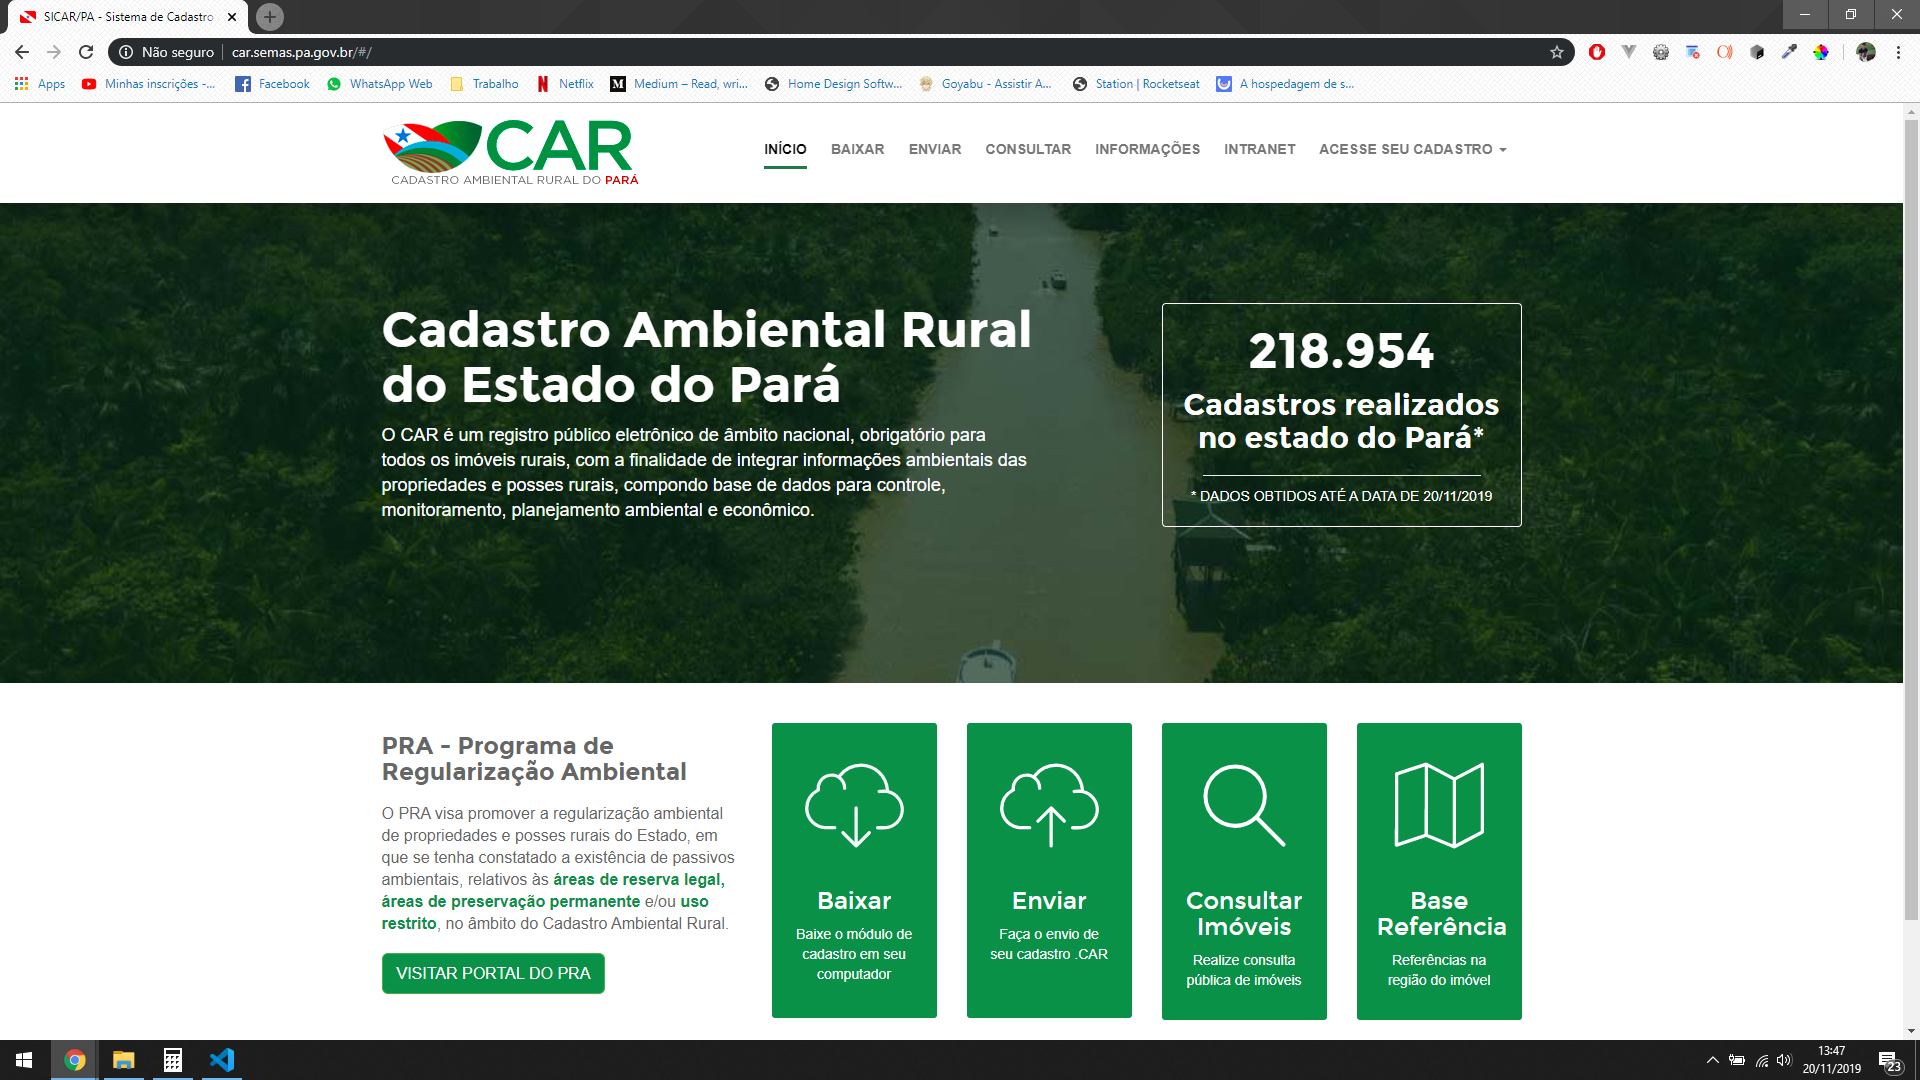
\includegraphics[scale=0.3]{SICAR}\\  % o 0.9 indica 90% do tamanho original
% pdfLaTeX aceita figuras no formato PNG, JPG ou PDF
% figuras vetoriais podem ser exportadas para eps e depois convertidas para pdf usando epstopdf
{\small Fonte: http://car.semas.pa.gov.br/#/} %Fonte da imagem
\label{fig:exemplo} %rotulo para refencia
\end{figure}

O projeto do SICAR tinha como objetivo informar e controlar os cadastros ambientais rurais feitos no estado do pará, sendo necessária algumas integrações com os módulos do SICAR federal e as Centrais ligadas ao PRA.

\begin{figure}[H]
\centering
\caption{PRA-OFF} %legenda
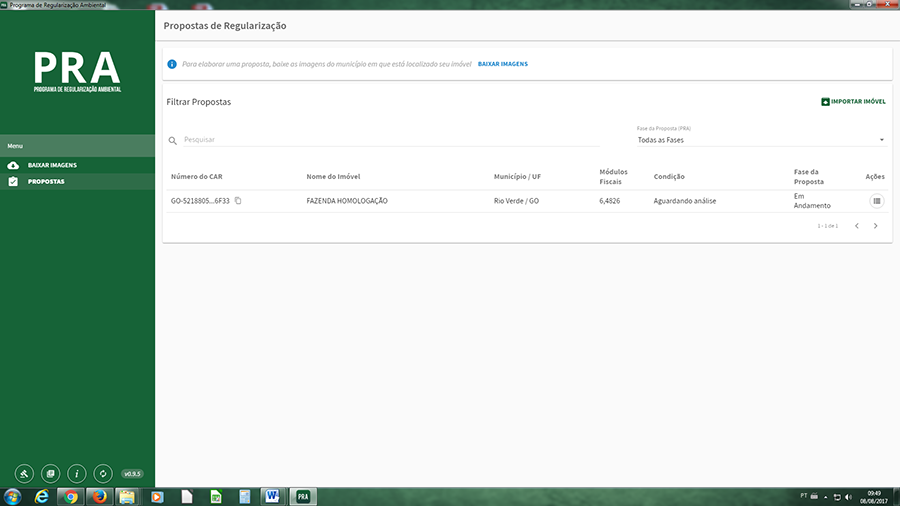
\includegraphics[scale=0.5]{pra-off}\\  % o 0.9 indica 90% do tamanho original
% pdfLaTeX aceita figuras no formato PNG, JPG ou PDF
% figuras vetoriais podem ser exportadas para eps e depois convertidas para pdf usando epstopdf
{\small Fonte: http://www.cprh.pe.gov.br/Controle_Ambiental/Sistema%20Nacional%20de%20Cadastro%20Ambiental%20Rural%20-%20Sicar/PRA/43052%3B53356%3B480802%3B0%3B0.asp} %Fonte da imagem
\label{fig:exemplo} %rotulo para refencia
\end{figure}

Já o projeto do PRA, não era possíveis tais integrações, pois ele era um modulo offline, sendo possível a utilização sem internet. Para o desenvolvimento do mesmo, foi necessário estudar sobre electron, uma ferramenta que possibilita criar modulos web em aplicações offiline.

Após 5 meses a equipe foi quebrada em duas e então foi feita uma redistribuição de projetos e acabei indo para a tribo Runners. Os projetos principais que contribui durante esse período foram o Consulta Publica - PARÁ e relatórios do PRA.

\begin{figure}[H]
\centering
\caption{Consulta publica} %legenda
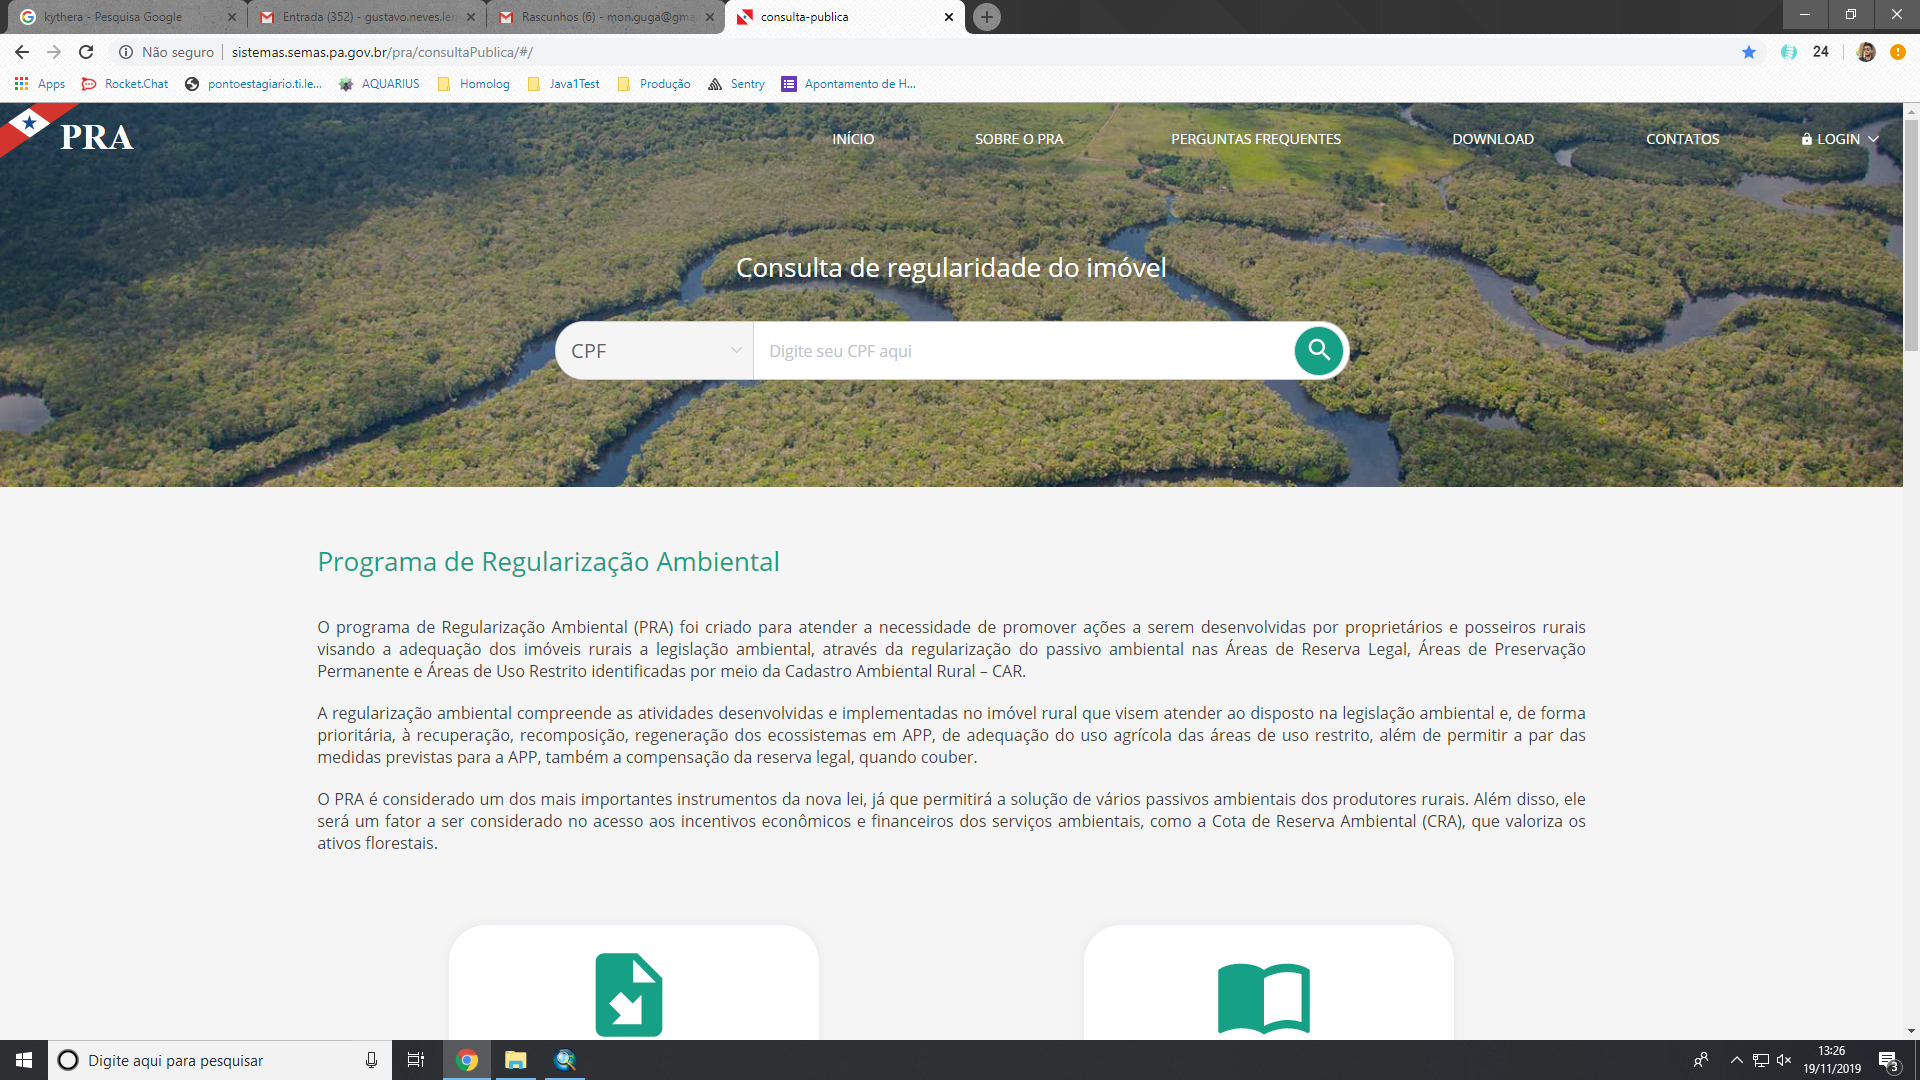
\includegraphics[scale=0.22]{consulta-publica}\\  % o 0.9 indica 90% do tamanho original
% pdfLaTeX aceita figuras no formato PNG, JPG ou PDF
% figuras vetoriais podem ser exportadas para eps e depois convertidas para pdf usando epstopdf
{\small Fonte: http://sistemas.semas.pa.gov.br/pra/consultaPublica/#/} %Fonte da imagem
\label{fig:exemplo} %rotulo para refencia
\end{figure}

O projeto consulta publica foi o primeiro projeto que tive como objetivo a refatoração, pois o projeto era antigo, utilizava uma das primeiras versões de VueJs no frontend e tinha o layout bem ruim.
Foi a primeira obrigação que tive total responsabilidade, tinha que migrar todo o sistema para VueJs 2.0 e refatorar o frontend.

Como era minha primeira experiencia com o framework VueJs, o projeto foi bem demorado, tive suporte do meu time que me tutoreava sobre arquitetura, padrões de projetos, boas praticas.
Para melhor aprendizado meu e um controle sobre códigos ruins, todas modificações feitas por mim sempre passavam por um Code Review e só quando aprovadas, eram enviadas para o projeto. 

O projeto consulta publica tinha como objetivo mostrar para os proprietários de imoveis rurais suas áreas desmatadas, se seus imoveis estavam de acordo com as regularizações ambientais e informações gerais sobre a geometria e hidrografia do terreno.


\begin{figure}[H]
\centering
\caption{Relatórios do PRA} %legenda
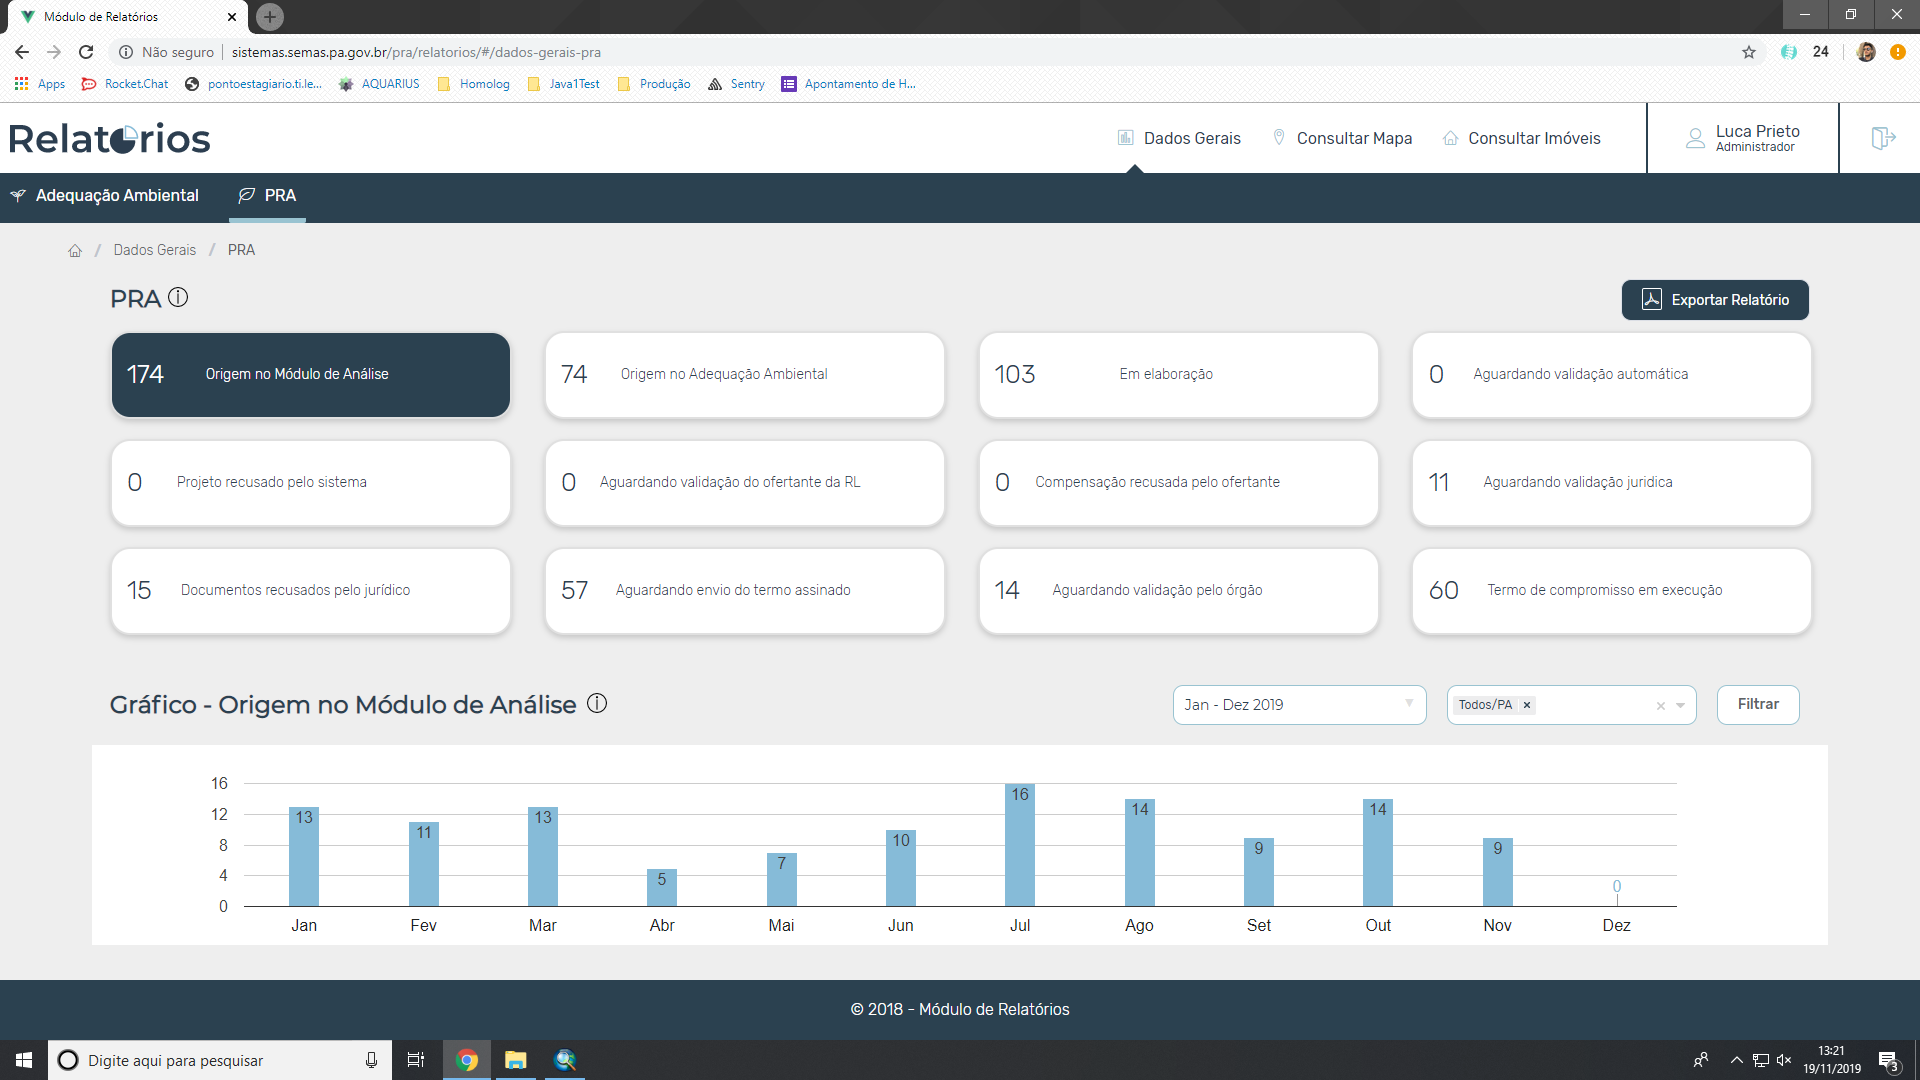
\includegraphics[scale=0.22]{relatorios-pra}\\  % o 0.9 indica 90% do tamanho original
% pdfLaTeX aceita figuras no formato PNG, JPG ou PDF
% figuras vetoriais podem ser exportadas para eps e depois convertidas para pdf usando epstopdf
{\small Fonte: http://sistemas.semas.pa.gov.br/pra/relatorios/#/dados-gerais-adequacao-ambiental} %Fonte da imagem
\label{fig:exemplo} %rotulo para refencia
\end{figure}

O projeto de relatórios foi o primeiro projeto que tive a honra de iniciar, com uma equipe formada de 4 pessoas (2 devs, uma tester e uma PO).
O projeto consistia em uma plataforma de relatórios sobre o Programa de regularização ambiental e Adequação ambiental.

A escolha da tecnologia foi deixada como escolha nossa, então pela ótima experiencias com VueJs e o alto desempenho do framework , escolhemos o mesmo para o frontend.
Porem pelo baixo conhecimento sobre backend, a escolha da tecnologia foi feita pelo outro Dev da equipe, que escolheu Spring Boot.
Como só tinha evoluído softwares e nunca começado um, houveram diversos gargalos no desenvolvimento, como criação de ambientes, scripts para automatização de deploy entre outros.

Porem apos 2 meses, fui transferido para uma equipe especial que não possuia tribo e que estava precisando de alguém com conhecimento em frontend e então me convocaram.
O projeto era uma POC(Prova de conceito) que uma empresa ligada a Agronomia havia comprado. Com prazos curtíssimos e complexidade alta, o projeto foi um dos mais difíceis que já havia trabalhado.
O projeto foi todo construído utilizando componentização, com o backend feito com uma arquitetura bem definida e documentada para que fosse possível evoluir sem dificuldade. Graças a esse começo bem estruturado o projeto ocorreu bem.

Após esse projeto, fui alocado na tribo Atlântida onde trabalhei juntamente com outro desenvolvedor em um projeto, o SEIRH-CMS.

\begin{figure}[H]
\centering
\caption{Seirh-CMS} %legenda
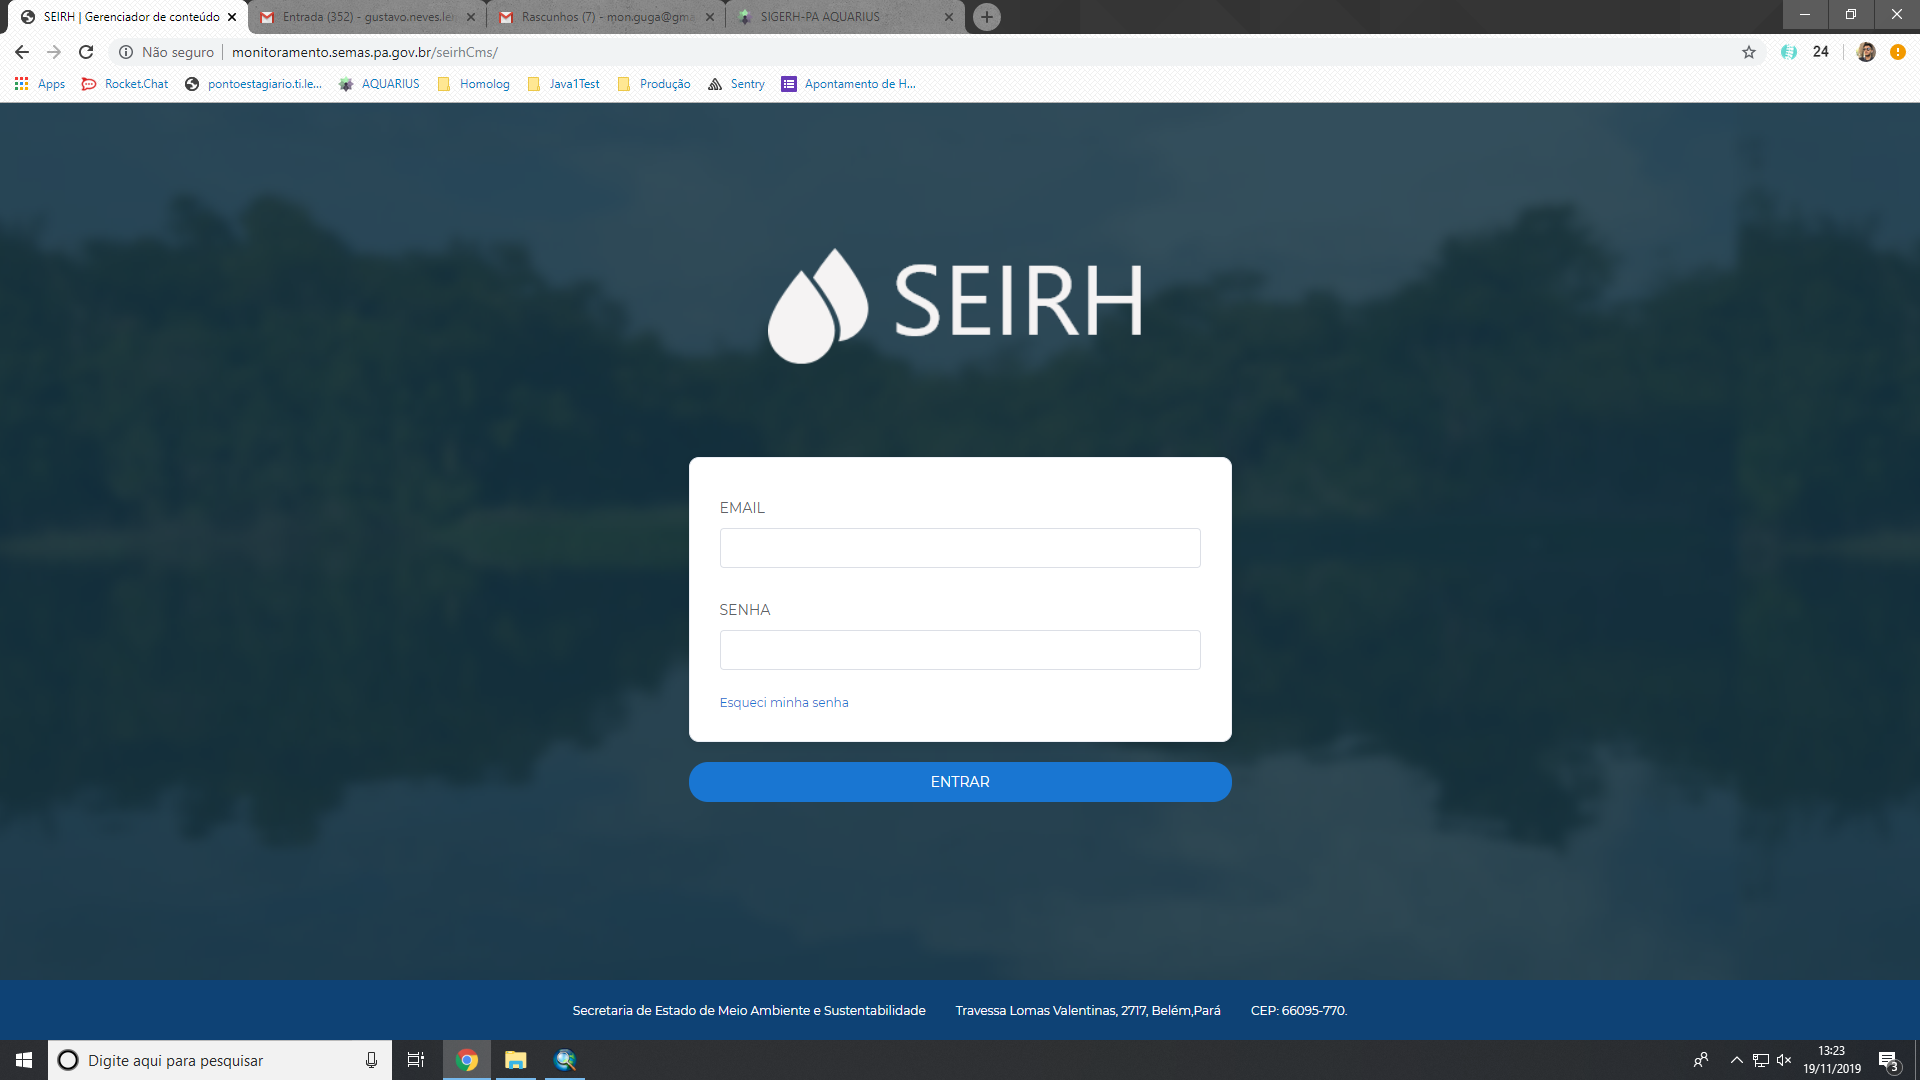
\includegraphics[scale=0.22]{seirh-cms}\\  % o 0.9 indica 90% do tamanho original
% pdfLaTeX aceita figuras no formato PNG, JPG ou PDF
% figuras vetoriais podem ser exportadas para eps e depois convertidas para pdf usando epstopdf
{\small Fonte: http://monitoramento.semas.pa.gov.br/seirhCms} %Fonte da imagem
\label{fig:exemplo} %rotulo para refencia
\end{figure}

O projeto do seirh-CMS era um gerenciador de conteúdo da aplicação seirh(Sistema Estadual de Informações Sobre Recursos Hídricos do Pará).
A plataforma web do seirh já existia, porem não havia comunicação com um backend, então seu conteúdo não era gerenciável, logo, havia a necessidade de uma refatoração total do sistema.

\begin{figure}[H]
\centering
\caption{Seirh} %legenda
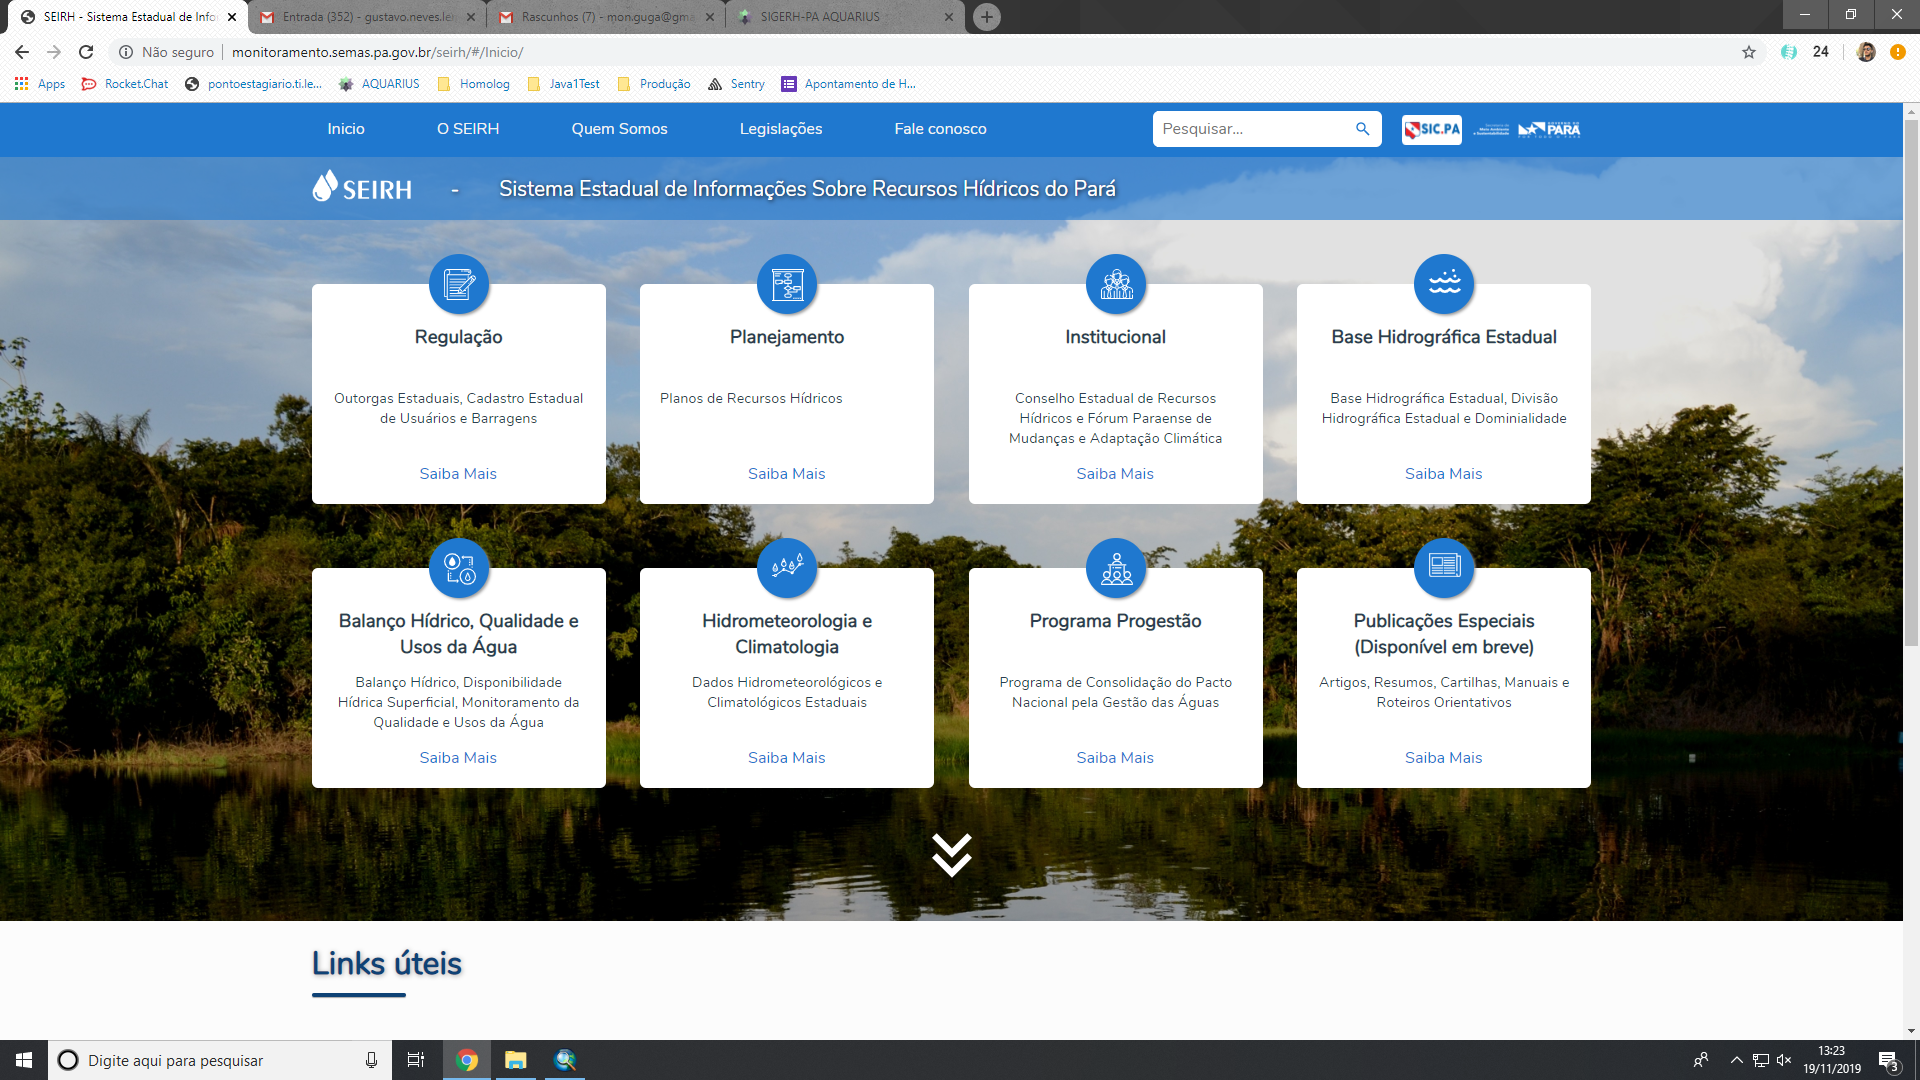
\includegraphics[scale=0.22]{seirh}\\  % o 0.9 indica 90% do tamanho original
% pdfLaTeX aceita figuras no formato PNG, JPG ou PDF
% figuras vetoriais podem ser exportadas para eps e depois convertidas para pdf usando epstopdf
{\small Fonte: http://monitoramento.semas.pa.gov.br/seirh} %Fonte da imagem
\label{fig:exemplo} %rotulo para refencia
\end{figure}

O prazo não diminui e então foi adicionado essa tarefa de refatoração ao nosso time.
Como já havia mais conhecimento sobre backend e toda tribo Atlântida ser constituída de desenvolvedores DotNet, resolvemos utilizar o framework DotNet Core 2.0, que 
provia diversas funcionalidades e atendia as nossas expectativas e necessidades.
Já o frontend continuou sendo feito com VueJs, uma vez que acabávamos de sair de projetos feitos com VueJs.

O projeto tinha como prazo 2 sprints(1 mes), um tempo muito curto e como era necessária a entrega, optamos por utilizar um quadro kanbam.
Foi minha primeira experiencia tomando liderança em prioridades das atividades, definição das atividades e organização no geral.

O projeto foi finalizado com excelência no prazo estipulado e graças a isso, fui realocado em um time que já trabalhava com DotNet e precisava de mais um desenvolvedor.

O projeto desta vez fazia parte de um grande complexo de plataformas que havia sido encomendado por uma empresa de agronomia e tinha muitos componentes de frontend parecidos.

Dai surgiu a iniciativa por parte minha e de outro desenvolvedor, de iniciar a construção do Design System da empresa.
Dai surgiu o Cria Design System, que é uma biblioteca de componentes UI para ReactJs.

Todos componentes eram criados pelo design do projeto, definido comportamentos e animações e depois desenvolvido. Para a visualização dos componentes separadamente, utilizamos o StoryBook,
que cria e organiza o catalogo de componentes e então para que essa biblioteca fosse compartilhada por toda empresa e não surgissem vários bugs, foram implementados testes automatizados para todos componentes e com uma nessesidade de cobertura de no minimo 80\%.

\begin{figure}[H]
\centering
\caption{Cria Design System} %legenda
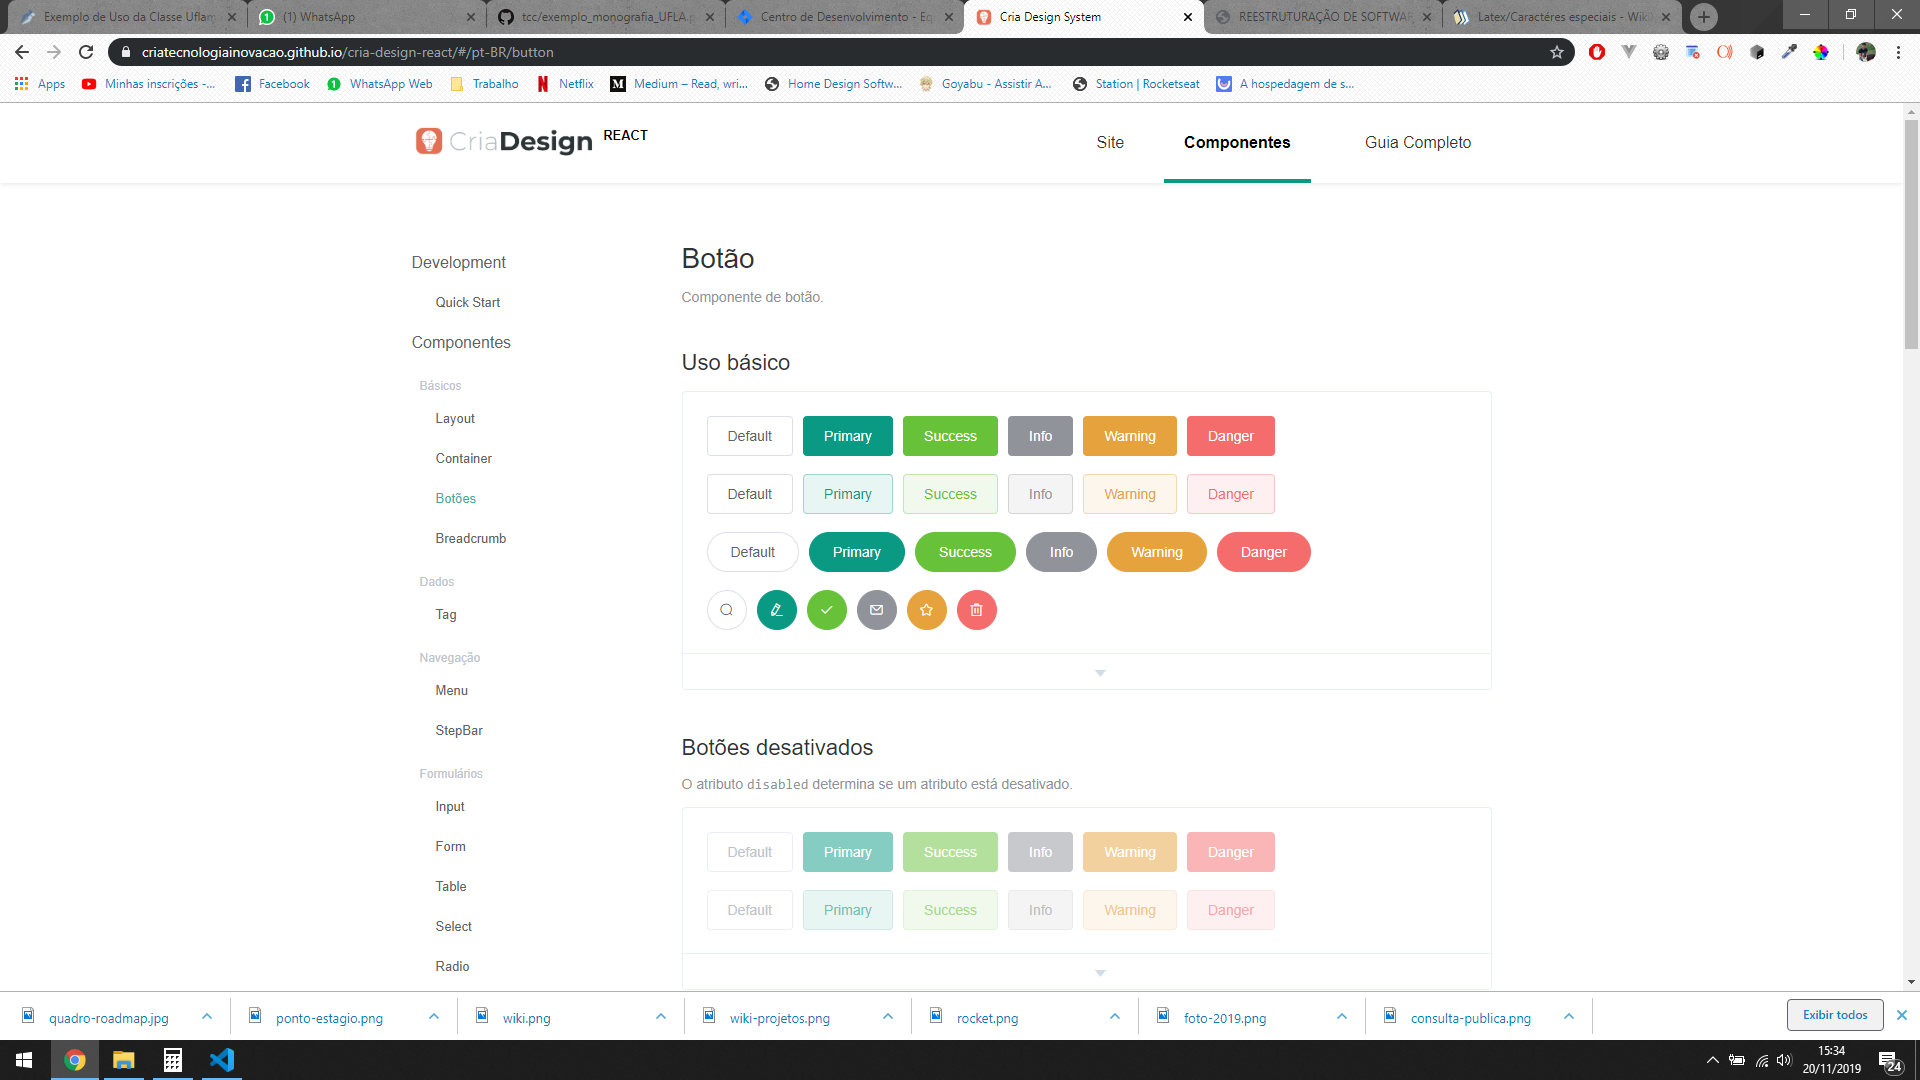
\includegraphics[scale=0.3]{cria-design}\\  % o 0.9 indica 90% do tamanho original
% pdfLaTeX aceita figuras no formato PNG, JPG ou PDF
% figuras vetoriais podem ser exportadas para eps e depois convertidas para pdf usando epstopdf
{\small Fonte: https://criatecnologiainovacao.github.io/cria-design-react/#/pt-BR/button} %Fonte da imagem
\label{fig:exemplo} %rotulo para refencia
\end{figure}

Apos ajudar com o começo do projeto e facilitar o desenvolvimento do mesmo, fui incorporado a uma equipe na mesma tribo e cuidava de alguns projetos como o SIOUT e Siger-pa.

\begin{figure}[H]
\centering
\caption{sigerpa} %legenda
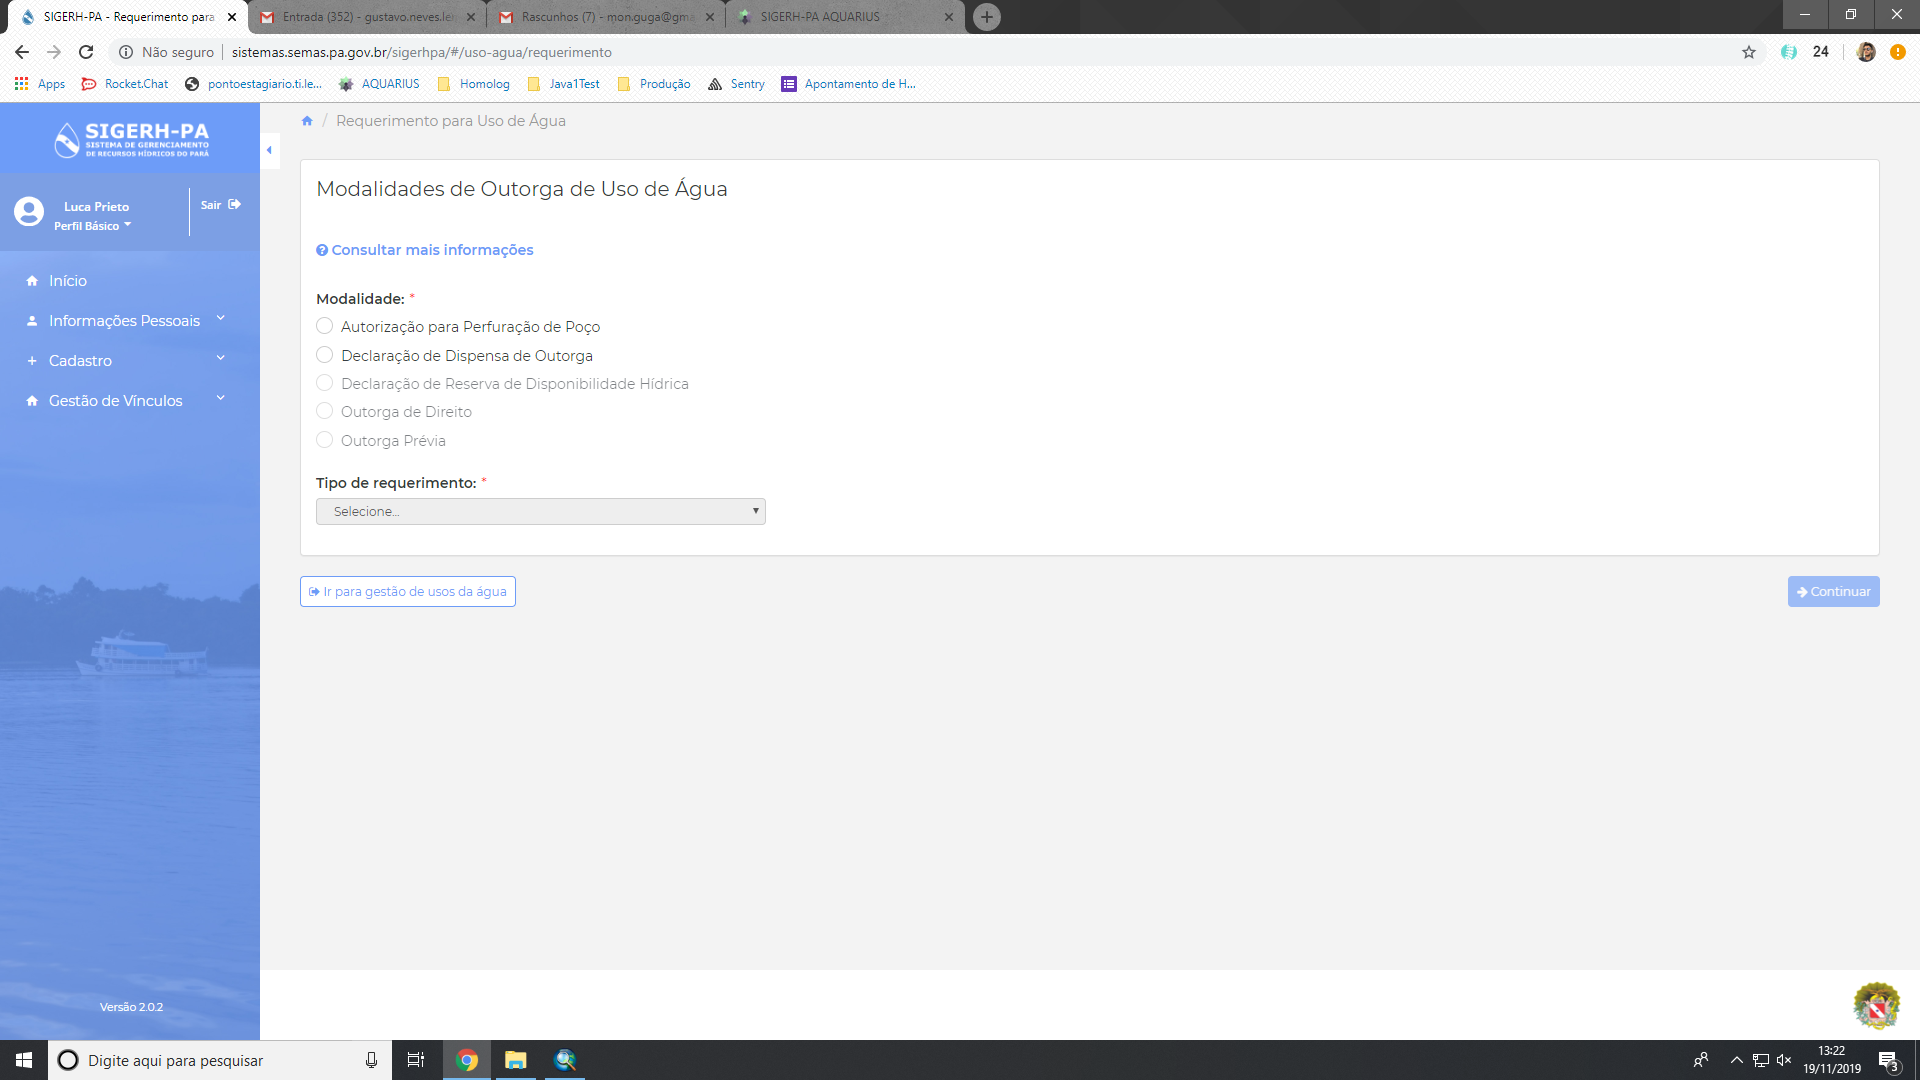
\includegraphics[scale=0.222]{sigerpa}\\  % o 0.9 indica 90% do tamanho original
% pdfLaTeX aceita figuras no formato PNG, JPG ou PDF
% figuras vetoriais podem ser exportadas para eps e depois convertidas para pdf usando epstopdf
{\small Fonte: http://sistemas.semas.pa.gov.br/sigerhpa/} %Fonte da imagem
\label{fig:exemplo} %rotulo para refencia
\end{figure}

O projeto do siger-pa(Sistema de Gerenciamento de Recursos Hídricos do Pará) é uma plataforma de cadastro e regularização de recursos hídricos(poços artesianos, nascentes e outros).
O projeto usava como backend o framework DotNet Framework 4.0 e como frontend AngularJs.

Até o fim do meu estágio, tive como tarefa evoluir e corrigir este sistema, que possuia vários problemas e alta complexidade por ser um sistema muito grande.

\chapter{CONCLUSÃO}
\label{cap:conclusao}

Toda minha experiência no LEMAF foi excepcional e de grande valia pro meu desenvolvimento profissional e pessoal, aprendendo a lidar com diversos problemas e pessoas.

A UFLA teve grande influencia na minha iniciativa no estagio, uma vez que a vaga me foi oferecida em um evento da SETI(Semana de Tecnologia da Informação) oferecido pela CompJunior\footnote{Empresa Junior do departamento de ciencia da computação} da UFLA e consegui a vaga apos faler na entrevista sobre alguns projetos que já havia desenvolvido pra disciplinas,
 sendo o que chamou a atenção do entrevistar o projeto que foi desenvolvido graças a matéria de Desenvolvimento Mobile, um aplicativo de chat com integração com Firebase\footnote{Um Baas (Backend as a Service) para aplicações Web e Mobile do Google}.
Quando iniciei o estágio, meu conhecimento era somente relacionado ao contexto acadêmico lecionado pela universidade até o quinto período de graduação, o que em sua grande maioria eram somente conhecimentos e teorias sobre otimizações e códigos de baixo nível.
Após alguns meses como estagiário, já possuía propriedade intelectual e autoridade para opinar em decisões estruturais de projetos, tecnologias e até mesmo estabelecer prazos, obviamente após inúmeros erros e muito estudo.
 
O estagio foi complementar a minha formação na UFLA assim como a UFLA complementava o estagio, varíos problemas eram solucionados graças a materias lecionadas na mesma e varias materias que cursei se tornaram simples pois já havia experiencia com aquilo.

Posso citar como exemplo as disciplinas de Banco de Dados, Sistemas Gerenciadores de Banco de Dados, Desenvolvimento Web, Modelagem e Implementação de Software, POO e muitas outras.

Os profissionais com os quais tive o prazer de trabalhar sempre foram muito agradáveis e solícitos, agregando muito valor ao meu desenvolvimento.

Devido aos problemas superados e projetos desenvolvidos no LEMAF, fui capaz de aprimorar minhas habilidades como desenvolvedor web e criar um bom portfólio, que me abriu diversas portas para o mercado de trabalho.
O estágio também me proporcionou uma visão abrangente de cargos e caminhos que poderei trilhar dentro da minha área de estudo, o que fez aumentar minhas oportunidades de escolhas e afirmar o que eu realmente tinha como desejo e vocação: ser desenvolvedor.

Posso afirmar com segurança que, os principais motivos da minha contratação na empresa Equals, meu emprego atual, foram minhas experiências com as tecnologias ReactJS, Spring e principalmente o desenvolvimento do Cria Design.

\begin{figure}[H]
\centering
\caption{Bilhete recebido da confraternização no fim de 2018} %legenda

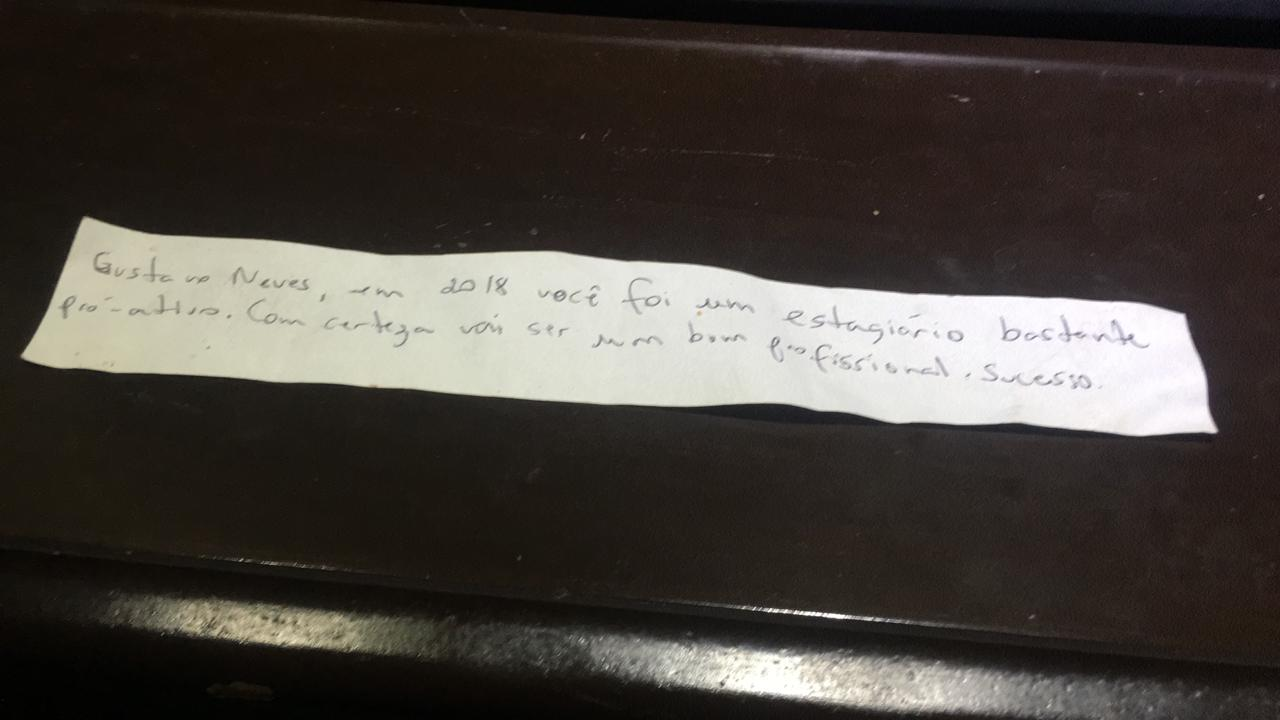
\includegraphics[scale=0.3]{agradecimento}\\  % o 0.9 indica 90% do tamanho original
% pdfLaTeX aceita figuras no formato PNG, JPG ou PDF
% figuras vetoriais podem ser exportadas para eps e depois convertidas para pdf usando epstopdf
\label{fig:exemplo} %rotulo para refencia
\end{figure}

Toda minha trajetória no laboratório foi muito prazerosa e produtiva. No meu ultimo dia de estágio, fui convidado a participar do podcast da empresa, onde compartilhei um pouco da minha experiência com os outros funcionários \footnote{\url{http://blog.ti.lemaf.ufla.br/2019/08/22/podcast-5/}}.


%==============================================================================
% Incluindo bibliografia
%\bibliographystyle{plain}             % estilo para labels em numeros
%\bibliographystyle{alpha}             % estilo para labels em iniciais
\bibliographystyle{abntex2-alf}           % estilo para referências usando ABNT, 
                                       % precisa instalar o abntex para usar!!!

%inclui Referências Bibliográficas
%inclui Referências Bibliográficas
\referencias
\bibliography{refbib}			% arquivo exemplo refbib.bib
%==============================================================================
% Incluindo anexos num1erados com letras maiusculas.
%\apendices
\apendice{O que são apêndices}
\label{cap:apendice}

Um apêndice é um suporte elucidativo e ilustrativo do texto principal. Sua função é agrupar elementos que são úteis à compreensão do texto e que, no entanto, podem ser apresentados à parte sem prejuízo à compreensão. É útil para a apresentação de modelagens, diagramas extensos, listagens de código-fonte de programas e demais elementos que o autor julgar necessário à complementação do tema abordado no texto principal.


%==============================================================================
% Fim do texto
\end{document}
